\documentclass{beamer}
\usepackage{tikz}
\usepackage{svg}
\usepackage{amsmath}
\usepackage{graphicx}
\usepackage{fontawesome}


\makeatother
\setbeamertemplate{footline}
{
\leavevmode%
\hbox{%
\begin{beamercolorbox}[wd=.3\paperwidth,ht=2.25ex,dp=1ex,center]{author in head/foot}%
    \usebeamerfont{author in head/foot}\insertshortauthor
\end{beamercolorbox}%
\begin{beamercolorbox}[wd=.6\paperwidth,ht=2.25ex,dp=1ex,center]{title in head/foot}%
    \usebeamerfont{title in head/foot}\insertshorttitle
\end{beamercolorbox}%
\begin{beamercolorbox}[wd=.1\paperwidth,ht=2.25ex,dp=1ex,center]{date in head/foot}%
    \insertframenumber{}
\end{beamercolorbox}}%
\vskip0pt%
}

\makeatletter
\setbeamertemplate{navigation symbols}{}


% setting some colors for the theme
\setbeamercolor{palette primary}{fg=black,bg=white}
\setbeamercolor{palette secondary}{fg=black,bg=white}
\setbeamercolor{structure}{fg=black,bg=white}
\setbeamercolor{title in head/foot}{fg=black,bg=white}
\setbeamercolor{date in head/foot}{fg=black,bg=white}


% definition of the title page template
\defbeamertemplate*{title page}{mytheme}[1][]
{%
\begin{tikzpicture}[remember picture,overlay]
    \filldraw[white]
    (current page.north west) --
    (current page.north east) --
    ([xshift=0cm,yshift=-2cm]current page.north east)  --
    ([xshift=0cm,yshift=-2cm]current page.north west) -- cycle
    ;
    \node[opacity=0.2] at ([xshift=-4.6cm,yshift=0cm]current page.north east)
    {
\includegraphics[width=22cm]{fhnw_title.png}};
    \node[text=black,anchor=south west,font=\sffamily\LARGE,text width=.6\paperwidth]
    at ([xshift=-100pt,yshift=-1cm]current page.center)
    (title)
    {\raggedright\inserttitle};

    \node[text=black,anchor=south west,font=\sffamily\small,text width=.6\paperwidth]
    at ([xshift=-100pt,yshift=-1.5cm]current page.center)
    (institute)
    {\raggedright\insertinstitute};

    \node[anchor=west]
    at ([xshift=-100pt,yshift=1cm]current page.south east)
    {
\includegraphics[height=1.00cm]{fhnw_small.png}};
    \node[text=black,font=\large\sffamily,anchor=south west]
    at ([xshift=30pt,yshift=0.5cm]current page.south west)
    (date)
    {\insertdate};
    \node[text=black,font=\large\sffamily,anchor=south west]
    at ([yshift=5pt]date.north west)
    (author)
    {\insertauthor};
\end{tikzpicture}%
}

% remove navigation symbols
\setbeamertemplate{navigation symbols}{}

% definition of the symbols used in itemize
\newcommand\mysymbol{%

\begin{tikzpicture}[xscale=0.85]
    \draw[black, thick]  circle (3.0 pt);
\end{tikzpicture}%
}

% definition of the itemize templates
\defbeamertemplate*{itemize item}{mysymbol}{\small\raise0.5pt\hbox{\mysymbol}}
\defbeamertemplate*{itemize subitem}{mysymbol}{\footnotesize\raise0.5pt\hbox{\mysymbol}}
\defbeamertemplate*{itemize subsubitem}{mysymbol}{\footnotesize\raise0.5pt\hbox{\mysymbol}}

\title[Nat64 und Casting für IML]{Zwischenbericht Team 11: \protect\\ Nat64 und Casting für IML}
\author{B. Meyer, M. Romanutti}
\date{\today}

\institute{FHNW}

\begin{document}

    % Title
    \begin{frame}[plain]
        \maketitle
    \end{frame}

    % Agenda
    \begin{frame}
        \frametitle{Agenda}
        \begin{itemize}
            \item Idee
            \item Lexikalische Syntax
            \item Grammatikalische Syntax
            \item Kontext- und Typen-Einschränkungen
            \item Vergleich mit Java
            \item Beispielprogramme
        \end{itemize}

    \end{frame}

    % Idee
    \begin{frame}
        \frametitle{Idee}
        \centering
        Nat64\footnote{positive Zahlen bis 64 bits und 0} + Casting = \faRocket
    \end{frame}

    % Lexikalische Syntax
    \begin{frame}
        \frametitle{Lexikalische Syntax}
        \begin{itemize}
            \item Neuer Datentyp
            \item Zusätzlicher Operator für Casting
        \end{itemize}
        \vspace{30}
        {\hspace{15}
\includegraphics[width=8cm]{listing_1.png}}

    \end{frame}

    % Grammatikalische Syntax
    \begin{frame}
        \frametitle{Grammatikalische Syntax}
        \framesubtitle{Neuer Datentyp}
        {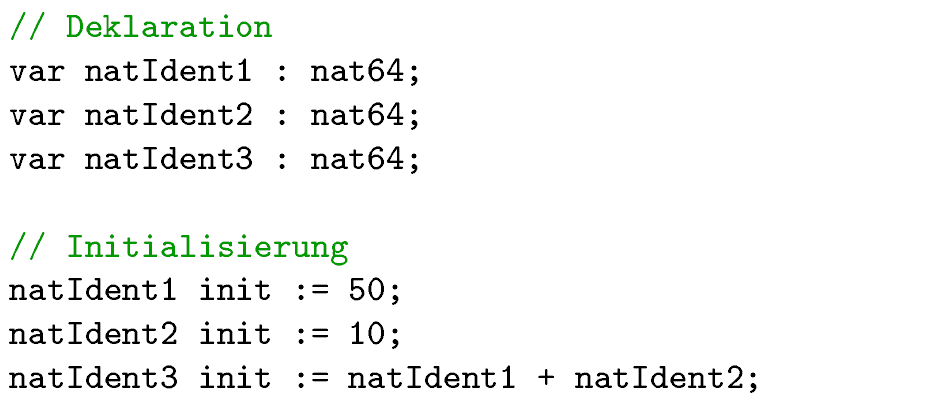
\includegraphics[width=8cm]{listing_2.png}}
    \end{frame}

    % Grammatikalische Syntax
    \begin{frame}
        \frametitle{Grammatikalische Syntax}
        \framesubtitle{Casting}
        {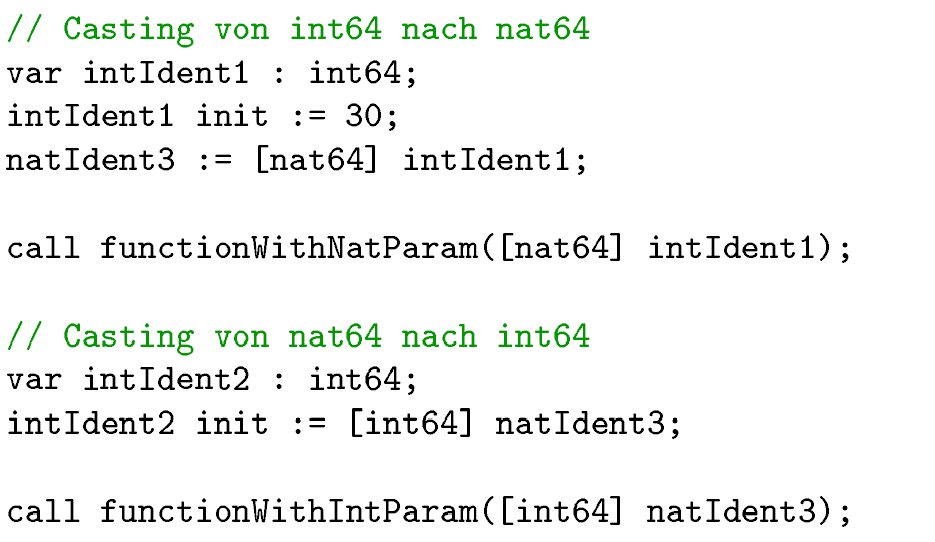
\includegraphics[width=8cm]{listing_3.png}}
    \end{frame}

    % Grammatikalische Syntax
    \begin{frame}
        \frametitle{Grammatikalische Syntax}
        \framesubtitle{Compiler-Error}
        {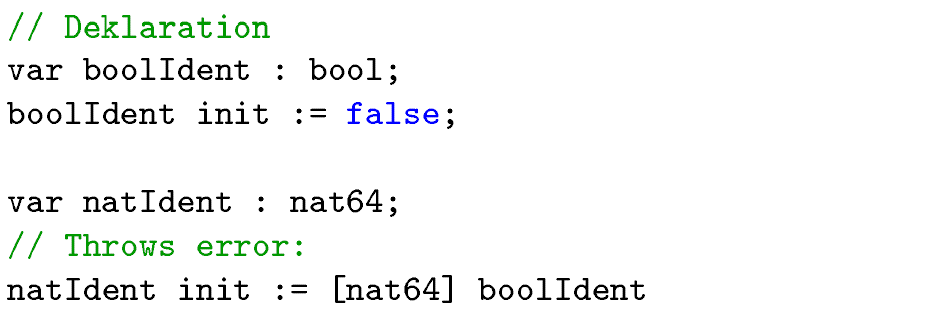
\includegraphics[width=8cm]{listing_4.png}}
    \end{frame}

    % Grammatikalische Syntax
    \begin{frame}
        \frametitle{Grammatikalische Syntax}
        \framesubtitle{Änderungen an der bestehenden Grammatik}

        \begin{itemize}
            \item Zusätzlicher Operator \texttt{castOpr} für Casting
            {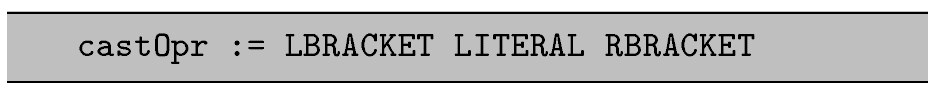
\includegraphics[width=8cm]{listing_5.png}}
            \item Ergänzung von Nichtterminal-Symbol \texttt{factor}
            {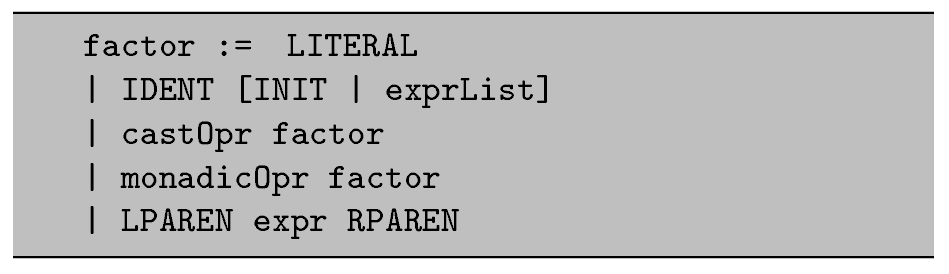
\includegraphics[width=8cm]{listing_6.png}}
        \end{itemize}
        \vspace{30}
    \end{frame}

    % Kontext- und Typen-Einschränkungen
    \begin{frame}
        \frametitle{Kontext- und Typen-Einschränkungen}
        \begin{itemize}
            \item Unterstützt folgende Castings:
            {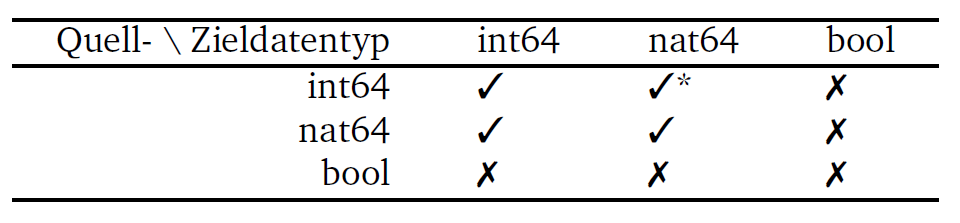
\includegraphics[width=8cm]{listing_7.png}}
            \item Definiertes Verhalten in Spezialfällen:
                \begin{itemize}
                    \item Werteüberlauf: Maximaler Wert wird verwendet
                    \item Negative Werte: Werte werden absolut interpretiert
                    \item Rest bei Divison: Nachkommastellen werden ignoriert
                \end{itemize}
        \end{itemize}
        \vspace{30}
    \end{frame}

    % Vergleich mit Java
    \begin{frame}
        \frametitle{Vergleich mit Java}
        \begin{itemize}
            \item Unterschiedliches Verhalten für Initialisierung und fortlaufende Berechnungen
            \begin{itemize}
                \item Error falls Wertebereich bei Initialisierung überschritten wird
                \item Implizite Umwandlung falls Wertebereich bei fortlaufender Berechnung überschritten wird
            \end{itemize}
            \item Werteüberlauf führt zu entsprechendem Wert auf Zahlenkreis
        \end{itemize}
        \vspace{30}
    \end{frame}

    % Beispielprogramme
    \begin{frame}
        \frametitle{Beispielprogramme}
        \framesubtitle{Addition}
        {\includegraphics[width=8cm]{listing_8.png}}
        \vspace{30}
    \end{frame}

    \begin{frame}
        \frametitle{Beispielprogramme}
        \framesubtitle{Casting}
        {\includegraphics[width=8cm]{listing_9.png}}
        \vspace{30}
    \end{frame}

\end{document}
